\chapter{Introduction}\label{chap:intro}
\glsaddall
\thispagestyle{empty}


\section{Lentilles gravitationnelles fortes de type galaxie-galaxie}\label{sec:lentilles gravitationnelles}


Fritz \citet{Zwicky1937}, suivant les calculs publiés par \citet{Einstein1936} et la première observation 
de l'effet de déviation gravitationnelle de la lumière par \citet{Eddington1919}, 
est largement reconnu comme étant le premier à observer correctement qu'une lentille gravitationnelle, et en particulier 
l'anneau d'Einstein \citep{Chwolson1924},
est un phénomène particulièrement riche en information\footnote{ 
        Les travaux pionniers de Franti\v{s}ek \citet{Link1936,Link1937}, largement ignorés dans la littérature anglo-saxonne, %\citep{Valls-Gabaud2006}, 
        offrent déjà une perspective riche et détaillée sur le phénomène des lentilles gravitationnelles au moment où \citet{Zwicky1937} publie 
        ses observations. 
        En particulier, \citet{Link1936} décrit la magnification d'une étoile lors du passage derrière un objet massif et 
        observe que les amas globulaires et les galaxies sont des candidats idéaux pour une recherche systématique du 
        phénomène.
        }. 
L'article de \citet{Zwicky1937} articule précisément deux idées centrales qui nous motivent encore aujourd'hui à 
étudier ces objets. En premier lieu, une lentille gravitationnelle est un télescope naturel, de sorte qu'un tel 
système nous permettrait en principe d'étudier l'image lentillée de la source en arrière-plan avec une résolution beaucoup plus grande que nos instruments 
nous le permettraient si l'effet de lentille n'avait pas eu lieu. En second lieu, la déflexion de l'image de la source 
est directement proportionnelle à la masse (gravitationnelle) de la lentille. 
\begin{equation}\label{eq:Taille Lentille}
        \theta_E = \sqrt{\frac{4 G M}{c^{2} D}} \simeq 3\left( \frac{M}{M_{\odot}} \right)^{\frac{1}{2}} \left( \frac{D}{1\, \mathrm{Gpc}} \right)^{-\frac{1}{2}}\, \mu\mathrm{as} \hspace{1cm} \left\{D \equiv \frac{D_{\ell} D_s}{D_{\ell s}}\right\}\, .
\end{equation}
Par exemple, une galaxie typique de masse $M\sim 10^{11} M_{\odot}$, à une distance caractéristique $D= 3 \, \mathrm{Gpc}$ produirait des 
images de la source séparées par $2 \theta_E \sim 1''$. C'est cette observation qui intéressait particulièrement 
\citet{Zwicky1937b}, insatisfait par les méthodes pour mesurer la masse des nébuleuses extragalactiques (galaxies) 
de l'époque, basées largement sur des comparaisons de la luminosité totale de ces galaxies avec $L_\odot$, la luminosité du Soleil, 
ou des courbes de rotation képlériennes.\footnote{
\citet{Zwicky1937b} a estimé la masse de l'amas de Coma à $\gtrsim 4.5\times  10^{13}M_\odot$ avec le théorème du viriel. 
Cette limite inférieure est un très bon estimé de 
la valeur acceptée aujourd'hui, dérivée avec les effets de lentilles faibles produites par l'amas 
sur l'image des galaxies environnantes, soit $5^{+4.3}_{-2.1} \times 10^{14}\, h^{-1}_{70}\,M_\odot$\citep{Gavazzi2009}.
} 

\citet{Einstein1936} considérait l'éventualité d'observer ces systèmes comme étant extrêmement 
improbable, pointant vers les limitations instrumentales de l'époque. En effet, les télescopes terrestres étaient 
largement limités par l'effet de \textit{seeing} atmosphérique, soit la distorsion de l'image causée par la turbulence de 
l'atmosphère.

\begin{figure}[tb!]
        \centering
        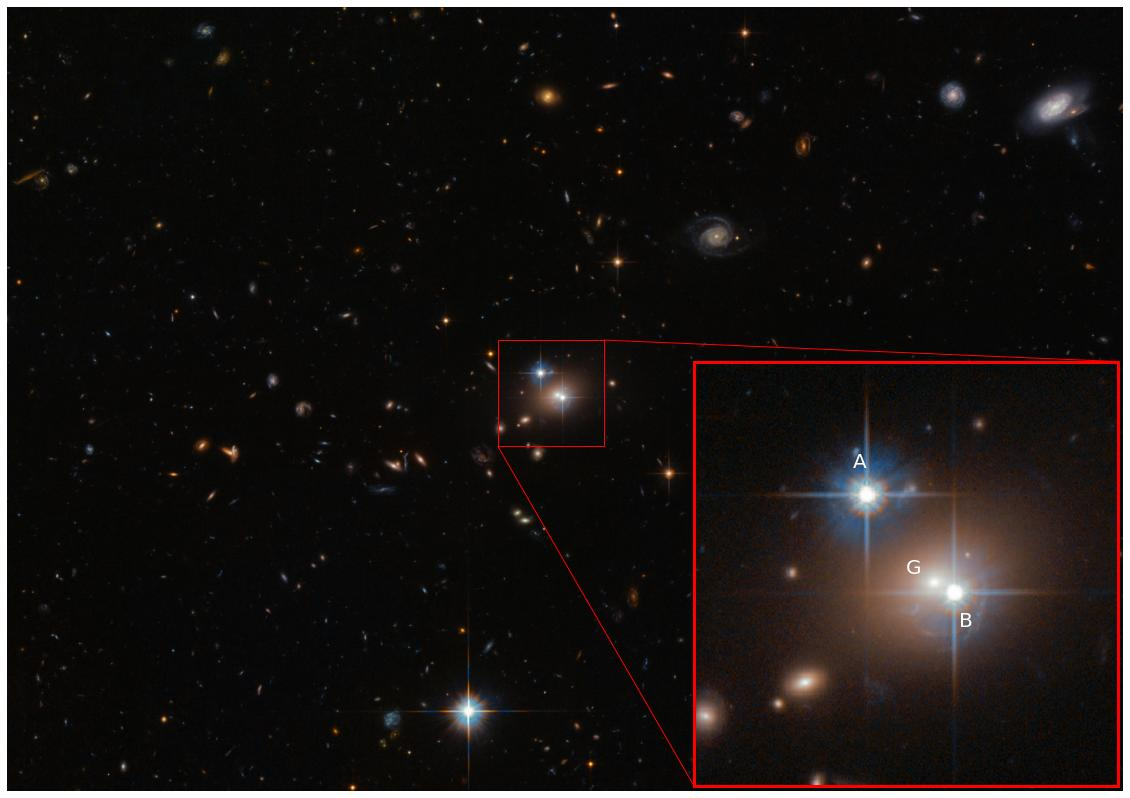
\includegraphics[width=0.8\textwidth]{figures/zoomed_in_qso0957}
        \caption{Le quasar double (QSO 0957+561 A et B) et la galaxie-lentille (G) imagée par le télescope spatial Hubble. 
        Crédit: ESA/Hubble et NASA, enlargissement par AA.}
        \label{fig:doubel quasar}
\end{figure}

Dû à cette difficulté pratique, 
la première lentille gravitationnelle est découverte seulement plusieurs décennies après la prédiction de leur existence par \citet{Walsh1979}, 
suivant l'identification de deux spectres radios de quasars identiques, QSO 0957+561 A et B, séparés par $5.7$ secondes d'arcs
et capturés avec le télescope radio Mark II à l'observatoire Jodrell Bank. 
Les spectres partagent la même magnitude, $m=17$, le même décalage vers le rouge, $z=1.405$, et possèdent des détails 
chimiques suspicieusement semblables. Ces coïncidences suggèrent fortement que ces deux spectres sont des copies d'un seul objet, soit un noyau 
actif d'une galaxie en arrière-plan, produite par l'effet de lentille gravitationnelle d'une galaxie en avant-plan, invisible dans le 
domaine radio à une fréquence de $966\,\mathrm{MHz}$. Cette hypothèse est rapidement confirmée par 
l'observation optique de la galaxie-lentille ($z=0.355$) avec l'observatoire Palomar \citep{Young1980}\footnote{Simulténament 
observé et confirmé par le télescope de $2.2\, m$ de l'Université d'Hawaii au mont Mauna Kea \citep{Stockton1980}.}, 
ainsi que la modélisation de sa distribution de masse, de son environnement 
et des angles de déflexion qui causeraient l'apparition d'une image double du quasar \citep{Young1981,Falco1991}

À la suite de cette découverte fortuite, l'étude des lentilles gravitationnelles est devenue un sujet d'étude 
particulièrement riche et prometteur pour la cosmologie \citep{Blandford1992,Bartelmann2010,Treu2010}. 
Par exemple, les lentilles gravitationnelles permettent de mesurer 
la constante de \citet{Hubble1929}, $H_0$, qui mesure le taux de l'expansion de l'Univers au temps présent. Les deux méthodes principales 
pour faire cette mesure à l'aide des lentilles gravitationnelles sont la caractérisation de la courbe de lumière des supernovas lentillées 
\citep{Refsdal1964,Kelly2015,Goobar2017} 
et la surveillance décennale de quasars lentillés 
\citep[e.g.][]{Vanderriest1989,Wong2020}. 



\begin{figure}[tb!]
        \centering
        \begin{subfigure}[t]{0.45\textwidth}
                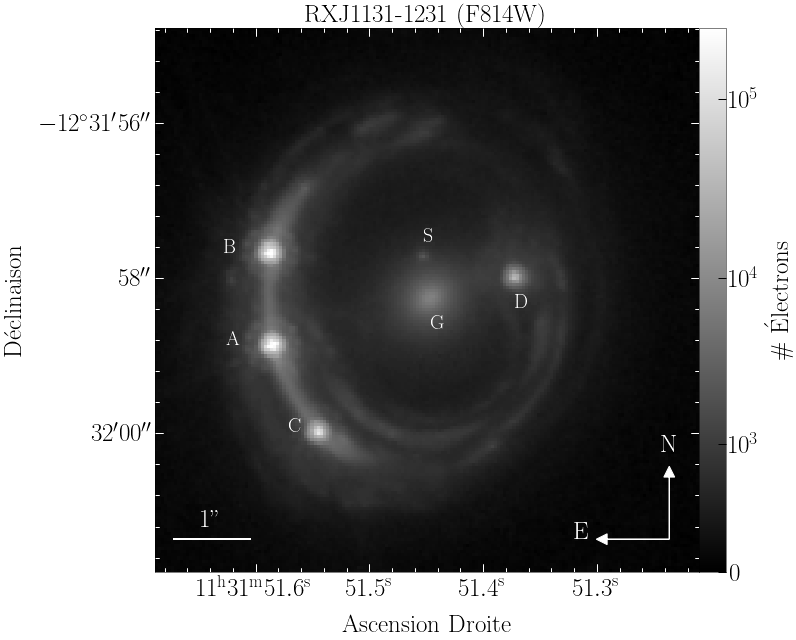
\includegraphics[width=\linewidth]{figures/rxj1131} 
                \caption{Quasar quadruplement lentillé (A, B, C et D) par une galaxie (G). L'image de la galaxie hébergeant le quasar 
                        est déformée tangentiellement, formant un anneau d'Einstein. Image prise par HST avec le filtre F814W.}
                \label{fig:rxj1131}
        \end{subfigure}
        ~
        \begin{subfigure}[t]{0.45\textwidth}
                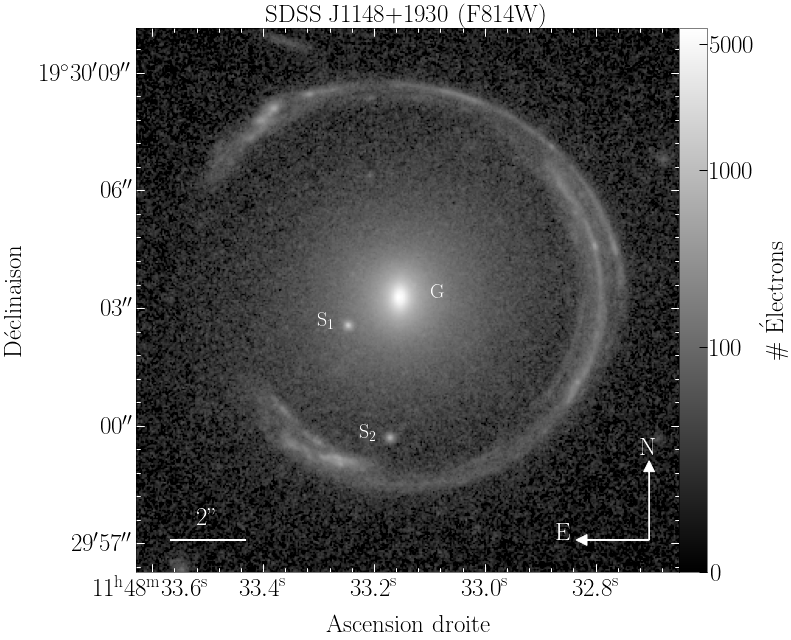
\includegraphics[width=\linewidth]{figures/sdssj1148} 
                \caption{Le fer à cheval cosmique, soit l'image d'une proto-galaxie à très haut décalage vers le rouge 
                        ($z=2.379$) fortement magnifiée et déformée par une galaxie elliptique lumineuse en infrarouge (G) exceptionnellement massive 
                        \citep[${5.2\times 10^{12}\, h_{72}^{-1}\, M_\odot}$,][]{Schuldt2019}. 
                 Image prise par HST avec le filtre F814W.}
                \label{fig:sdssj1148}
        \end{subfigure}
        \caption{Lentilles gravitationnelles de type galaxie-galaxie.}
        \label{fig:important lenses}
\end{figure}
 

De ce fait, plusieurs programmes ont été entamés pour trouver des lentilles gravitationnelles. Le programme 
\textit{Sloan Lens ACS Survey} \citep[SLAC,][]{Bolton2005,Bolton2006}, basé sur la recherche systématique de spectres de galaxies de type ETG\footnote{\textit{Early-Type Galaxies}} 
avec des lignes d'absorption à un décalage vers le rouge plus grand que les lignes d'émission, 
est un des programmes les plus réussis, ayant mené à la découverte 
confirmée de plus de $150$ lentilles gravitationnelles de type galaxie-galaxie \citep{Bolton2008,Shu2017}. Les programmes 
basés sur la recherche visuelle d'images doubles, triples, d'arcs ou d'anneaux \citep[e.g.][]{Faure2008} dans les champs larges et profonds comme 
COSMOS \citep{Koekemoer2007,Scoville2007}, connaissent aujourd'hui une renaissance nourrie par les succès récents de l'apprentissage profond 
pour la perception visuelle \citep{Krizhevsky2012}. Cette nouvelle approche a déjà mené à la découverte de plus de $1000$ lentilles 
gravitationnelles \citep{Petrillo2017,Huang2021}, et est projetée de découvrir plus de $10^{5}$ systèmes grâce aux nouvelles expéditions 
à champs larges comme les observatoires Rubin \citep{lsst2009} et Euclid \citep{Euclid2010}.


Le sujet du chapitre \ref{chap:censai} se concentre sur le défi de développer un algorithme pour modéliser la distribution de masse et 
la morphologie de la source. Cet algorithme est dédié à analyser le nombre grandissant
de lentilles gravitationnelles connues, dans toute leur complexité et dans un temps à l'échelle humaine. 
Dans la section qui suit, je dérive les équations centrales qui nous permettent 
d'étudier les lentilles gravitationnelles de type galaxie-galaxie.
Mon traitement est largement inspiré 
des manuels de références de \citet{Meneghetti2013,Congdon2018}. 


\subsection{Les angles de déflexion}

Supposons qu'un photon est sur une trajectoire parallèle à l'axe de 
visée $\mathbf{e}_{\parallel}$ d'un observateur sur Terre. 
Supposons de plus que la source d'un champ gravitationnel $\Phi$ est située sur l'axe de visée, 
ce qui a pour effet de courber la 
trajectoire de ce photon entre son point d'origine $A$ et son point d'arrivée $B$.
On définit l'angle de déviation comme la déviation totale de cette trajectoire 
dans la direction perpendiculaire à l'axe de visée de l'observateur. 
De façon générale, cette déviation s'écrit
\begin{equation}\label{eq:intro alpha}
        \boldsymbol{ \alpha} = - \int_{\lambda_A}^{\lambda_B} \ddot{\mathbf{x}} \times \mathbf{e}_{\parallel} d\lambda\, ,
\end{equation}
où $\lambda$ paramétrise la trajectoire du photon $\mathbf{x}(\lambda)$. 
Le signe négatif nous indique qu'on prend la perspective de l'observateur. 

La trajectoire d'un photon obéit au 
principe de Fermat, qui stipule que la lumière suit une trajectoire qui extrémise
la durée du parcours entre deux points. 
Dans le langage du calcul 
des variations, la variation de la durée s'écrit
\begin{equation}\label{eq:Fermat}
        \delta T =  \delta \int_{A}^{B} n(\mathbf{x}(\ell)) \frac{d\ell}{c}= 0\, ,
\end{equation}
où $\ell$ est un élément de longueur sur la trajectoire et $n$ est un indice de réfraction.
Pour déterminer l'indice de réfraction du champ gravitationnel d'une galaxie, 
on doit utiliser le formalisme de la relativité générale. Selon le principe 
d'équivalence (fort), 
l'effet d'un champ gravitationnel est localement 
indistinguable d'une accélération causée par la courbure 
d'un espace-temps décrit par 
une métrique $g_{\mu \nu}$. 
La trajectoire d'un photon se trouve alors en cherchant 
les géodésiques de cet espace-temps. 
On fait l'approximation 
que le potentiel $\Phi$ d'une galaxie est celui d'un gaz parfait, c'est-à-dire 
qu'il satisfait une équation de Poisson
\begin{equation}\label{eq:Poisson}
       \grad^{2}\Phi = 4\pi G \rho .
\end{equation} 
Dans la limite où ce potentiel est faible $\displaystyle \frac{2\Phi}{c^{2}} \ll 1$, la 
métrique $g_{\mu \nu}$ est décrite par une expansion au premier ordre autour de la 
métrique de Minkowsky %$\eta_{\mu\nu}$
\begin{equation}\label{eq:metrique}
        ds^2 = g_{\mu\nu}dx^{\mu}dx^{\nu} \approx \left( 1 + \frac{2\Phi}{c^{2}} \right)c^{2}dt^{2} - \left( 1 - \frac{2\Phi}{c^{2}} \right)d\mathbf{x}^{2}.
\end{equation} 
Puisqu'un photon suit une géodésique de l'espace-temps $ds^{2} = 0$, on peut déterminer 
l'indice de réfraction en réarrangeant l'équation \eqref{eq:metrique}
\begin{equation}\label{eq:n}
        n \equiv c \left( \frac{\lVert d \mathbf{x} \rVert}{dt}  \right)^{-1} \approx  1 - \frac{2\Phi}{c^{2}}.
\end{equation} 
En réécrivant l'élément de longueur $d\ell$ en termes du 
paramètre de la trajectoire
$
        d\ell = \left\lVert\frac{d  \mathbf{x} }{d\lambda} \right\rVert d\lambda,
$
on peut réécrire l'équation \eqref{eq:Fermat} sous la forme
\begin{equation}\label{eq:Fermat2}
        \delta \int_{\lambda_A}^{\lambda_B} n(\mathbf{x}) \lVert \mathbf{\dot{x}} \rVert d\lambda = 0.
\end{equation} 
Par correspondance avec la fonctionnelle de l'action 
$J(x) = \int_{\lambda_0}^{\lambda_1} \mathcal{L}(\lambda,\, x,\,\dot{x}) d\lambda$, on trouve que 
le lagrangien de la trajectoire s'écrit 
$
        \mathcal{L} = n(\mathbf{x})  \sqrt{\dot{x}^{2}}.
$
La trajectoire qui satisfait \eqref{eq:Fermat} 
est une solution des équations d'Euler-Lagrange
\begin{equation}\label{eq:EulerLagrange}
        \frac{d }{d \lambda} \frac{\partial \mathcal{L}}{\partial \dot{\mathbf{x}}} - \frac{\partial \mathcal{L}}{\partial \mathbf{x}} = 0.
\end{equation} 
On a donc
\begin{equation}\label{eq:EulerLagrange2}
        \frac{d }{d \lambda} n \frac{\dot{\mathbf{x}}}{\lVert \dot{\mathbf{x}} \rVert}- \lVert \dot{\mathbf{x}} \rVert \grad n = 0 ,
\end{equation} 
Puisque le choix du paramètre $\lambda$ est libre, on peut le choisir tel 
que $\lVert \dot{\mathbf{x}} \rVert = 1$ en tout point de la trajectoire. Ainsi,
\begin{align}
        \nonumber
        \frac{d }{d \lambda} n \dot{\mathbf{x}} -  \grad n &= 0 \\
\label{eq:EulerLagrange3}
        \implies n \ddot{\mathbf{x}} + (\grad n \cdot \dot{\mathbf{x}}) \dot{\mathbf{x}} - \grad n &= 0
\end{align} 

À ce point de la dérivation, on utilise l'approximation de Born. 
C'est-à-dire qu'on approxime la trajectoire 
du photon comme une ligne droite sur l'axe de visée $\mathbf{e}_{\parallel}$. 
Cette approximation est justifiée 
dans le contexte des lentilles gravitationnelles de type galaxie-galaxie, 
puisque les angles de déviation sont généralement de 
l'ordre de l'arcseconde ou plus petit. 
Comme le vecteur $\dot{\mathbf{x}}$ est tangent à la trajectoire du photon, les termes $ \propto \dot{\mathbf{x}} \times \mathbf{e}_{\parallel} $ s'annulent. 
En subsitutuant l'indice de réfraction par \eqref{eq:n} dans $\mathbf{e}_{\parallel} \times \eqref{eq:EulerLagrange3}$, on obtient
\begin{equation}\label{eq:sol}
        \ddot{\mathbf{x}} \times \mathbf{e}_{\parallel} = \frac{1}{n} \grad_\perp n = \grad_\perp \log n
        \approx -\frac{2}{c^{2}}\grad_{\perp} \Phi\,,
\end{equation} 
où $\grad_\perp$ est un gradient selon les coordonnées perpendiculaires à $\mathbf{e}_\parallel$.
On note que le facteur 2 qui apparaît dans l'équation \eqref{eq:sol} est un 
effet qui vient de la relativité générale. Ce facteur corrige la solution 
que l'on aurait obtenue avec une dérivation classique (newtonienne).


On est maintenant en mesure de calculer l'angle de déviation. 
J'introduis le paramètre d'impact $\boldsymbol{\xi}$ qui est la distance perpendiculaire entre 
la position d'origine du photon sur le plan de la lentille  
et l'axe de visée (voir Figure \ref{fig:cartoon}).
Dans le cas où le potentiel est généré par une masse $M$ ponctuelle, c.-à-d.\ qu'on 
suppose $\rho = M\delta^{3}(\mathbf{x})$, où $\delta $ est la fonction delta de Dirac, 
alors le potentiel qui satisfait l'équation de Poisson \eqref{eq:Poisson} est 
la fonction de Green 
$\displaystyle \Phi = -\frac{GM}{\sqrt{ \xi^{2} + z^{2}}}$, où $z$ est la coordonnée 
sur l'axe de visée. L'équation \eqref{eq:intro alpha} se réécrit finalement comme 
\begin{align}
\nonumber
        \boldsymbol{ \alpha}(\boldsymbol{ \xi} ) &= -\frac{2GM}{c^{2}} \int_{-\infty }^{\infty }  \frac{\partial}{\partial \boldsymbol{\xi} }\frac{1}{(\xi^{2} + z^{2})^{1/2}}dz \\
\label{eq:deflection approx}
        \implies \boldsymbol{ \alpha}(\boldsymbol{ \xi})  &= \frac{4GM}{c^{2}  \xi^{2} } \boldsymbol{ \xi}
\end{align} 
Cette solution se généralise naturellement à un profil de masse quelconque en assumant 
qu'il s'exprime comme une somme d'éléments de masse $dm = \Sigma d^{2}\boldsymbol{ \xi}'$, 
où $\Sigma = \int \rho dz$ est une densité surfacique de masse. 
L'angle de déviation total mesuré à un point $\boldsymbol{\xi} $ est alors une convolution 
sur tout le plan de la lentille (mince) puisque l'équation \eqref{eq:deflection approx} dépend 
linéairement de la masse $M$:
\begin{equation}\label{eq:alpha physique}
        \boldsymbol{ \alpha} (\boldsymbol{ \xi} ) = \frac{4 G}{c^{2}} 
        \int_{\mathbb{R}^{2}} \Sigma (\boldsymbol{ \xi} ')
        \frac{\boldsymbol{ \xi}  - \boldsymbol{ \xi} '}{\lVert \boldsymbol{ \xi}  - \boldsymbol{ \xi} ' \rVert^{2}}d^{2}\boldsymbol{ \xi} '
\end{equation} 

\begin{figure}[tb!]
        \centering
        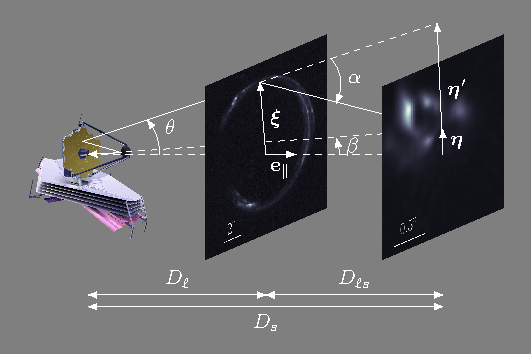
\includegraphics[width=0.8\textwidth]{figures/lensing_cartoon}
        \caption{Schéma d'une lentille gravitationnelle.}
        \label{fig:cartoon}
\end{figure}

L'angle de déviation est une quantité cruciale pour résoudre une lentille gravitationnelle 
puisqu'il décrit une transformation des coordonnées angulaires du plan de la lentille ($\boldsymbol{ \theta} $) 
vers les coordonnées angulaires du plan de la source ($\boldsymbol{ \beta} $). 
On assume que les distances entre l'observateur et la lentille $D_{\ell}$, entre l'observateur et la source $D_s$ et entre la lentille et la source $D_{\ell s}$, 
sont beaucoup plus grandes que les distances perpendiculaires à l'axe de visée $\boldsymbol{ \xi} $ ou $\boldsymbol{ \eta}$ 
(voir figure \ref{fig:cartoon}). 
Cette approximation est justifiée pour les objets qui nous intéressent,
pour lesquels les distances parallèles à l'axe de visée sont généralement 
de l'ordre du Gpc, alors que les distances perpendiculaires sont généralement 
de l'ordre du kpc; soit 6 ordres de grandeur de différence.
Ainsi, on peut faire un argument géométrique (euclidien) 
\begin{align}
\nonumber
       D_{s} \boldsymbol{ \theta} &= \boldsymbol{ \eta}' \\   
\nonumber
       D_{s} \boldsymbol{ \beta} &= \boldsymbol{ \eta} \\   
\nonumber
       D_{\ell s} \boldsymbol{ \alpha} &= \boldsymbol{ \eta}' - \boldsymbol{ \eta}  \\   
\label{eq:lens equation}
       \implies D_s \boldsymbol{ \beta} &= D_s \boldsymbol{ \theta} - D_{\ell s} \boldsymbol{ \alpha}   
\end{align} 
La dernière relation est l'équation maîtresse qui nous permet de tracer les rayons lumineux d'une source 
vers un détecteur fictif dans nos simulations. 

On notera que cette relation reste valide pour un Univers courbe et/ou en expansion 
(c.-à-d.\ décrit par une géométrie non euclidienne), 
à condition qu'on utilise une notion de distance qui satisfait, par définition, la relation trigonométrique euclidienne
\begin{equation}\label{eq:diameter angular distance}
       D \equiv \frac{\xi}{\theta}\, ,
\end{equation} 
où $\xi$ est la taille physique d'un objet placé à une certaine distance de l'observateur, et $\theta$ est l'angle solide sous-tendu 
par cet objet. Pour un Univers décrit par la métrique de Friedmann-Lemaître-Robertson-Walker,
la notion de distance qui respecte la définition \eqref{eq:diameter angular distance} est la distance du diamètre angulaire. 
En pratique, on peut exprimer $D$ en termes du décalage vers le rouge des photons émis par l'objet, $z$. 
On note $a(z)$ le facteur d'échelle lorsque le photon est émis par la source et $a(0)$ le facteur d'échelle au moment présent ($z=0$).
Pour un Univers plat \citep[voir les manuels de référence][]{Coles2002,Dodelson2003,Bartelmann2004}
\begin{align}
        D_z &= c a(z) \underbrace{\int_{a(z)}^{a(0)} \frac{da}{a \dot{a}}}_{\strut\mathclap{\text{distance comobile}}}; \\[2ex]
                \nonumber
              &= \frac{c a(z)}{H_0} \int_{a(z)}^{a(0)} \frac{da}{\sqrt{\Omega_{r,0} + \Omega_{m,0} a  + \Omega_{\Lambda,0}a^{4}}}; \\
              \label{eq:dang}
              &= \frac{c}{H_0(1 + z)} \int_{0}^{z} \frac{dz'}{\sqrt{\Omega_{r,0}(1 + z')^{4} + \Omega_{m,0} (1 + z')^{3} + \Omega_{\Lambda,0} }}\, .
\end{align}
On a utilisé la relation entre le facteur d'échelle, $a$, et le décalage vers le rouge, $a = (1 + z)^{-1}$, pour obtenir l'équation \eqref{eq:dang} 
par un changement de la variable d'intégration. 
$\Omega_{r,0}$, $\Omega_{m,0}$ et $\Omega_{\Lambda, 0}$ sont les paramètres de densités, au temps présent, de la radiation, de la matière et de l'énergie sombre 
respectivement. 
%$\Omega_K = 1 - \Omega_0$ est le paramètre de courbure et 
$H_0$ est la constante de Hubble, soit le taux 
d'expansion de l'Univers au temps présent. La distance $D_{\ell s}$ se trouve simplement en ajustant les bornes de l'intégrale $\int_0^{z} \mapsto \int_{z_\ell}^{z_s}$.
La valeur des paramètres du modèle cosmologique $\Lambda$CDM obtenue par l'équipe \citet{PlanckCollaboration2018}
est rapportée dans l'annexe \ref{app:lcdm}.


Il est généralement pratique de travailler avec la forme adimensionnelle de l'équation \eqref{eq:lens equation}. 
On introduit la densité critique 
\begin{equation}\label{eq:densite critique}
        \Sigma_c = \frac{c^2}{4 \pi G}\frac{D_{s}}{D_{\ell s} D_\ell}\, ,
\end{equation} 
qui nous permet de définir la quantité qu'on nomme convergence $\displaystyle \kappa(\boldsymbol{ \theta} ) \equiv \frac{\Sigma(\boldsymbol{ \theta})}{\Sigma_c}$. 
On définit ainsi l'angle réduit 
\begin{equation}\label{eq:alpha adim}
        \hat{\boldsymbol{ \alpha}} (\boldsymbol{ \theta}) = \frac{1}{\pi}\int_{\mathbb{R}^{2}} \kappa(\boldsymbol{ \theta} )
        \frac{\boldsymbol{ \theta} - \boldsymbol{ \theta}'  }{\lVert \boldsymbol{ \theta} - \boldsymbol{ \theta}' \rVert  } d^{2}\boldsymbol{ \theta}'\, ,
\end{equation} 
qui satisfait l'équation de la lentille adimensionnelle 
\begin{equation}\label{eq:lens equation adim}
        \boldsymbol{ \beta} = \boldsymbol{ \theta} - \hat{\boldsymbol{ \alpha}}(\boldsymbol{ \theta})\, . 
\end{equation}


\section{Auto-encodeur variationnel}\label{sec:vae}
 
\subsection{Description du modèle}

Les auto-encodeurs variationnels (VAE) ont été introduits par \citet{Kingma2013} comme une approche 
pour inférer approximativement les variables latentes (ou cachées) qui contrôlent un certain processus génératif. 
Leur utilité est particulièrement marquée lorsque ce processus génératif est défini implicitement par un échantillon de données, 
soit un cas où la forme fonctionnelle de la distribution n'est pas connue a priori.
Dans cette section, j'introduis 
les concepts principaux reliés à ce type de modélisation. 
Le lecteur peut aussi se référer au livre blanc de \citet{Kingma2019}.

On définit $\mathbf{z}\in \mathbb{R}^{h}$ comme une variable latente et $\mathbf{x}\in \mathbb{R}^{m}$ ($m > h$) 
comme un exemple d'un échantillon de donnée $\mathcal{D} = \{\mathbf{x}^{(i)}\}_{i=1}^{N}$. 
Notre objectif est de modéliser la distribution, $p(\mathbf{x})$, implicitement décrite par notre échantillon. 
On définit une approximation de cette distribution, $p_\theta(\mathbf{x})$, caractérisée par une liste de paramètres $\theta$,
et on définit un processus génératif modélisé par la conditionnelle sur la variable cachée $p_\theta(\mathbf{x \mid \mathbf{z}})$. 
Déterminer $p_\theta$ directement est généralement difficile, voir impossible, si la dimensionnalité de $\mathbf{x}$ est grande 
($\mathrm{dim(\mathbf{x}}) \gtrsim 10^{4}$ pour des images). 
Pour contourner ce problème, on introduit une distribution variationnelle, $q_\phi(\mathbf{z} \mid \mathbf{x})$, dont le rôle est 
d'inférer la variable latente $\mathbf{z}$ associée à $\mathbf{x} \sim p_\theta(\mathbf{x} \mid \mathbf{z})$. 
En d'autres mots, $q_\phi(\mathbf{z} \mid \mathbf{x})$ est une approximation variationnelle de la distribution a posteriori $p_\theta(\mathbf{z} \mid \mathbf{x})$.
La notion de distance entre ces deux distributions est mesurée par la divergence de Kullback-Leibler $D_{\mathrm{KL}}(\cdot \KL \cdot) \geq 0$: 
\begin{align}
        \nonumber
       D_{\mathrm{KL}}(q_\phi(\mathbf{z} \mid \mathbf{x}) \KL  p_\theta (\mathbf{z} \mid \mathbf{x})) 
       &= \mathbb{E}_{q_\phi(\mathbf{z} \mid \mathbf{x})} \bigg[\log q_\phi(\mathbf{z} \mid \mathbf{x}) - \log p_\theta (\mathbf{z} \mid \mathbf{x}) \bigg]  \\
       \nonumber
       &= \mathbb{E}_{q_\phi(\mathbf{z} \mid \mathbf{x})} \bigg[\log q_\phi (\mathbf{z} \mid \mathbf{x}) -\log \frac{p_\theta(\mathbf{z}, \mathbf{x})}{p_\theta(\mathbf{x})} \bigg]  \\
       \label{eq:KL}
       &= \log p_\theta (\mathbf{x}) - \underbrace{\mathbb{E}_{q_\phi(\mathbf{z} \mid \mathbf{x})} \bigg[\log p_\theta(\mathbf{z}, \mathbf{x}) - \log q_\phi (\mathbf{z} \mid \mathbf{x}) \bigg]}_{\equiv \mathcal{L}_{\phi,\theta}(\mathbf{x})} \, .
\end{align} 

On remarque par cette manipulation que la distance $D_{\mathrm{KL}}$, en plus de mesurer la distance entre 
les deux distributions a posteriori (par définition), mesure aussi la différence entre le terme 
$\mathcal{L}_{\phi,\theta}(\mathbf{x})$, qu'on nomme limite inférieure sur l'évidence (de l'anglais 
\textit{evidence lower bound}: ELBO), et la distribution marginale qu'on cherche à modéliser, $p_\theta(\mathbf{x})$. 
L'objectif d'un modèle VAE est de maximiser la ELBO, $\mathcal{L_{\phi,\theta}}$. 
En observant l'équation \eqref{eq:KL}, on réalise que cet objectif 
nous permet d'améliorer le modèle d'inférence et le processus génératif simultanément.
En effet, la divergence KL est 
une quantité positive, donc maximiser la ELBO a pour effet de
\begin{enumerate}
        \item maximiser $p_\theta(\mathbf{x}) = \int p_{\theta}(\mathbf{x} \mid \mathbf{z}) p_{\theta}(\mathbf{z}) d\mathbf{z}$, ce qui suit de l'inégalité
                $\log p_\theta \geq \mathcal{L}_{\phi,\theta}(\mathbf{x})$ (améliore le processus génératif);
        \item minimiser $D_{\mathrm{KL}}(q_\phi(\mathbf{z} \mid \mathbf{x}) \KL  p_\theta (\mathbf{z} \mid \mathbf{x})) = \log p_\theta(\mathbf{x}) - \mathcal{L}_{\phi,\theta}(\mathbf{x})$ (améliore le processus d'inférence de $\mathbf{z}$).
\end{enumerate}

\begin{figure}[H]
        \centering
        \begin{tikzpicture}
                \node[circle, draw=black, minimum size=1cm] (z) at (0, 3) {$\mathbf{z}$};
                \node[circle, draw=black, minimum size=1cm] (x) at (0, 0) {$\mathbf{x}$};
                \draw[-{Latex[scale=2]}] (z) to (x);
                \draw[-{Latex[scale=2]}, in=225, out=135, dashed] (x) to (z);
                \node (phi) at (-2.5, 2.5) {$\phi$};
                \node (theta) at (2.5, 2.5) {$\theta$};
                \draw[rounded corners=0.5cm] (-1.5, -0.7) rectangle (1.5, 3.7);
                \draw[-{Latex[scale=2]}] (theta) to node[sloped, midway, below=5pt, fill=white, rectangle, draw=white, opacity=.8, text opacity=1] {$p_\theta(\mathbf{\mathbf{x} \mid \mathbf{z}})$} (x);
                \draw[-{Latex[scale=2]}] (theta) to node[sloped, midway, above=5pt, fill=white, rectangle, draw=white, opacity=.8, text opacity=1] {$p_\theta(\mathbf{z})$} (z);
                \draw[-{Latex[scale=2]}, dashed] (phi) to node[sloped, midway, above=5pt, fill=white, rectangle, draw=white, opacity=.8, text opacity=1] {$q_\phi(\mathbf{z} \mid \mathbf{x})$} (z); 
                \node at (1, -0.5) {$N$};
        \end{tikzpicture}
        \caption{Modèle graphique d'un VAE. Les flèches pleines indiquent le processus génératif, alors que les flèches pointillées indiquent le processus d'inférence.}
        \label{fig:vae encoder}
\end{figure}

\subsection{Le truc de reparamétrisation}
Le gradient de la ELBO par rapport aux paramètres variationnels, $\grad_{\phi,\theta}\mathcal{L}_{\phi,\theta}(\mathbf{x})$, 
est une quantité qu'on doit calculer pour faire usage d'algorithmes comme la grimpe de gradient stochastique 
pour maximiser la ELBO en termes de $\phi$ et $\theta$. 
Or, la liste de paramètres $\phi$ apparait dans la distribution de prélèvement pour calculer 
l'espérance mathématique $\mathbb{E}_{q_\phi(\mathbf{z} \mid \mathbf{x})}$ dans la ELBO \eqref{eq:KL}.
Cette opération n'a pas de dérivée formelle en termes de $\phi$. 

Pour résoudre ce problème, on utilise le truc de reparamétrisation \citep{Kingma2013}, 
qui consiste à exprimer la variable aléatoire latente $\mathbf{z} \sim q_\phi (\mathbf{z} \mid \mathbf{x})$ 
comme la transformation différentiable et inversible d'une variable aléatoire auxiliaire $\boldsymbol{\epsilon}$.
On considère le cas où $q_\phi(\mathbf{z} \mid \mathbf{x})$ et $p(\boldsymbol{ \epsilon})$ 
font partie de la famille gaussienne isotropique
\begin{align}
        \label{eq:p epsilon}
        \boldsymbol{\epsilon} &\sim \mathcal{N}(0, \bbone)\, ;\\
        %\label{eq:q phi}
        %q_\phi(\mathbf{z} \mid \mathbf{x}) &= \mathcal{N}(\boldsymbol{ \mu}_\phi (\mathbf{x}),\, \bbone \boldsymbol{\sigma}_\phi^{2}(\mathbf{x}))\, ;\\
        \label{eq:reparametrisation}
        \mathbf{z} &= \boldsymbol{\mu}_\phi + \boldsymbol{ \sigma}_\phi \odot \boldsymbol{ \epsilon}\, , 
\end{align} 
de sorte que 
\begin{equation}\label{eq:q phi}
        \mathbf{z} \sim q_\phi(\mathbf{z} \mid \mathbf{x}) = \mathcal{N}(\boldsymbol{ \mu}_\phi (\mathbf{x}),\, \bbone \boldsymbol{\sigma}_\phi^{2}(\mathbf{x}))\, .
\end{equation} 
$\odot$ symbolise le produit d'Hadamard, ou encore le produit élément par élément de vecteurs.
La reparamétrisation fait en sorte que les paramètres variationnels ne participent plus au processus de prélèvement, 
maintenant pris en charge par $\boldsymbol{ \epsilon} $.
Cette propriété est cruciale, car elle nous permet de prendre le gradient de la ELBO \eqref{eq:KL}. 
En effet, on peut maintenant échanger les opérateurs $\grad_{\phi,\theta}$ et ${\mathbb{E}_{q_\phi(\mathbf{z} \mid \mathbf{x})} = \mathbb{E}_{p(\boldsymbol{ \epsilon})}}$,
ce qui nous permet d'appliquer le gradient à l'intérieur de l'espérance mathématique.
De plus, $\phi$ décrit maintenant une fonction générique dont le rôle est d'inférer les 
paramètres de la distribution $q_\phi(\mathbf{z} \mid \mathbf{x})$
\begin{equation}
        \begin{aligned}
                f_\phi: \mathbb{R}^{m} &\rightarrow \mathbb{R}^{h} \times \mathbb{R}^{h}\\ \mathbf{x} &\mapsto (\boldsymbol{\mu},\, \log \boldsymbol{\sigma}^{2})
        \end{aligned}
\end{equation} 
En pratique, on peut construire une approximation de 
cette fonction avec un réseau de neurones convolutif lorsque $\mathbf{x}$ est une image, 
suivant le principe d'approximation universelle \citep{Cybenko1989,Hornik1991}. 

L'objectif d'entraînement de la fonction $f_\phi$ nécessite de manipuler la ELBO pour obtenir une 
divergence KL
\begin{align}
        \mathcal{L}_{\phi,\theta}(\mathbf{x}) &= \mathbb{E}_{q_\phi(\mathbf{z} \mid \mathbf{x})} \bigg[ \log p_\theta(\mathbf{z}, \mathbf{x}) - \log q_\phi (\mathbf{z} \mid \mathbf{x}) \bigg]\, ; \\
        \label{eq:final elbo}
         \implies \mathcal{L}_{\phi,\theta}(\mathbf{x})  &= 
         \underbrace{\mathbb{E}_{q_\phi(\mathbf{z} \mid \mathbf{x})} \bigg[ \log p_\theta(\mathbf{x} \mid \mathbf{z})\bigg]}_{\text{terme de reconstruction}}
         + \underbrace{
                \mathbb{E}_{q_\phi(\mathbf{z} \mid \mathbf{x})} \bigg[\log p_{\theta}(\mathbf{z}) - \log q_\phi (\mathbf{z} \mid \mathbf{x}) \bigg]
        }_{\equiv -D_{\mathrm{KL}}(q_\phi(\mathbf{z} \mid \mathbf{x})\, \KL\, p_\theta(\mathbf{z}))}\, .
\end{align} 
Pour déterminer la forme fonctionnelle de la divergence KL obtenue au second terme du membre droit de l'équation \eqref{eq:final elbo}, 
on stipule a priori que la distribution marginale des variables latentes 
devrait correspondre à une distribution normale isotropique
\begin{equation}\label{eq:latent distribution}
        p_{\theta}(\mathbf{z}) = \mathcal{N}(0, \bbone)
\end{equation}
La KL admet alors une solution fermée étant donné les familles paramétriques stipulées 
pour $p_\theta(\mathbf{z})$ \eqref{eq:latent distribution} et $q_\phi(\mathbf{z} \mid \mathbf{x})$ \eqref{eq:q phi}
\begin{equation}\label{eq:final KL}
        -D_{\mathrm{KL}}(q_\phi(\mathbf{z} \mid \mathbf{x})\, \KL\, p_\theta(\mathbf{z})) =
        \frac{1}{2}\sum_{j=1}^{h} (1 + [\log \boldsymbol{ \sigma}_\phi^{2} ]_j - [\boldsymbol{ \mu}_\phi ]_j - [\boldsymbol{ \sigma}_\phi^{2} ]_j)
\end{equation} 
Une dérivation de ce terme est donnée dans l'annexe B de \citet{Kingma2013}. 
%Cette solution se dérive directement par rapport à $\phi$. 
Le premier terme du membre droit de l'équation \eqref{eq:final elbo} 
est nommé \textit{terme de reconstruction} puisqu'il connecte avec l'objectif des fonctions 
de type auto-encodeur d'apprendre une représentation latente d'un échantillon de données.
La reconstruction s'accomplit en utilisant d'abord le modèle d'inférence 
$\mathbf{z}^{(1:L)} \overset{\mathrm{i.i.d}}{\sim} q_\phi(\mathbf{z} \mid \mathbf{x})$ 
pour obtenir un échantillon de représentations latentes à partir des équations \eqref{eq:p epsilon} à \eqref{eq:reparametrisation}, 
puis en utilisant le modèle génératif $\hat{\mathbf{x}}^{(i)} \sim p_\theta(\mathbf{x} \mid \mathbf{z}^{(i)})$ pour obtenir 
un échantillon de reconstructions $\mathbf{\hat{x}}^{(1:L)}$ de l'exemple originel $\mathbf{\mathbf{x}}$. 
Comme on a déjà une variable auxiliaire $\boldsymbol{ \epsilon} $ 
qui se charge de l'aspect génératif du modèle, on peut construire une approximation du 
modèle génératif avec une fonction générique des variables latentes 
${g_\theta: \mathbb{R}^{h} \rightarrow \mathbb{R}^{m};\, \mathbf{z}^{(i)} \mapsto \hat{\mathbf{x}}^{(i)}}$.
Encore une fois, un réseau de neurones convolutif est un choix pratique pour modéliser cette fonction 
dans le cas où $\mathbf{x}$ est une image. En général, on choisit une erreur quadratique moyenne pour modéliser le terme de reconstruction, 
de sorte que
\begin{equation}\label{eq:reconstruction}
        \mathbb{E}_{q_\phi(\mathbf{z} \mid \mathbf{x})} \bigg[
                \log p_\theta(\mathbf{x} \mid \mathbf{z})
        \bigg] 
        = -\frac{1}{L}\sum_{i=1}^{L} \lVert \mathbf{x} - \hat{\mathbf{x}}^{(i)} \rVert_2^{2}
\end{equation} 

\subsection{Principe du goulot d'information}

La fondation théorique des auto-encodeurs variationnels repose sur le principe plus général 
du goulot d'information \citep[BIP, de l'anglais \textit{bottleneck information principle:}][]{Tishby1999}. 
Dans cette sous-section, je décris rapidement certains concepts 
liés à la théorie de l'information de \citet{Shannon1948} 
pour justifier l'introduction d'un multiplicateur de 
Lagrange $\beta$ au terme de régularisation de la ELBO, ${-D_{\mathrm{KL}}(q_\phi(\mathbf{z} \mid \mathbf{x})\, \KL\, p_\theta(\mathbf{z}))}$.
Pour une discussion en profondeur, voir l'excellente revue sur l'utilisation de BIP dans le contexte de l'apprentissage 
machine par \citet{Goldfield2020} et le manuel de référence sur la théorie de l'information par \citet{Cover2006}.
\begin{figure}[thb!]
        \centering
        \resizebox{\linewidth}{!}{
        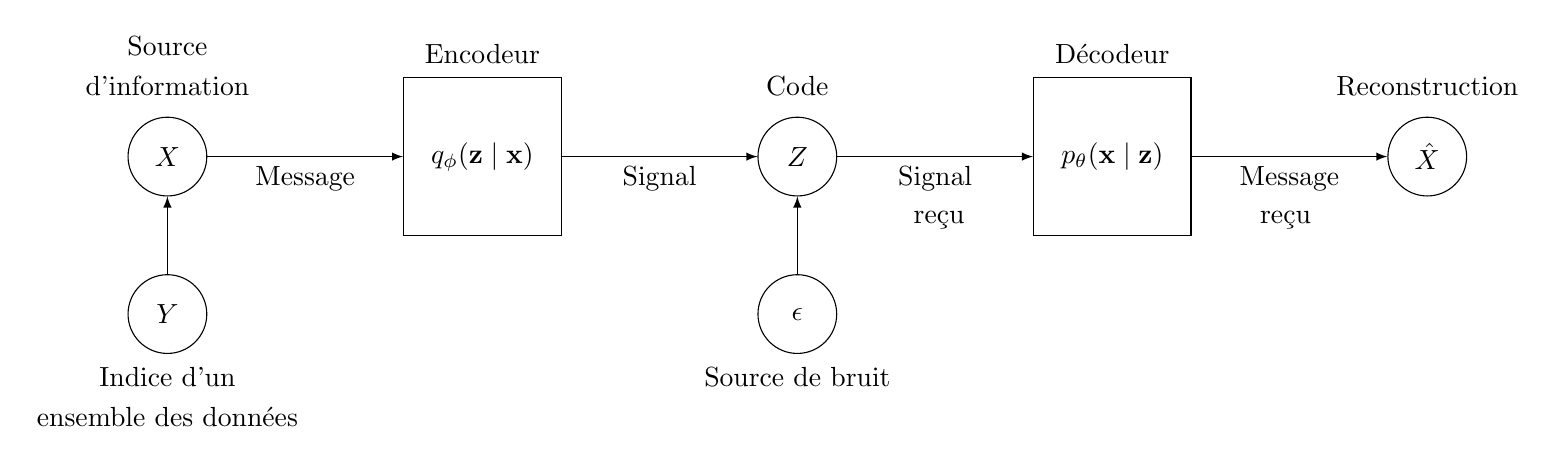
\begin{tikzpicture}
                \node at (-8, -2.8) {Indice d'un};
                \node at (-8, -3.3) {ensemble des données};
                \node[circle, draw=black, minimum size=1cm] (obj) at (-8, -2) {$Y$}; 
                \node at (-8, 1.4) {Source};
                \node at (-8, 0.9) {d'information};
                \node[circle, draw=black, minimum size=1cm] (x) at (-8, 0) {$X$}; 
                \node at (-4, 1.3) {Encodeur};
                \node[rectangle, draw=black, minimum width=2cm, minimum height=2cm] (encoder) at (-4, 0) {$q_\phi(\mathbf{z} \mid \mathbf{x})$}; 
                \node at (0, 0.9) {Code};
                \node[circle, draw=black, minimum size=1cm] (z) at (0, 0) {$Z$};
                \node[circle, draw=black, minimum size=1cm] (eps) at (0, -2) {$\epsilon$};
                \node at (0, -2.8) {Source de bruit};
                \node[rectangle, draw=black, minimum width=2cm, minimum height=2cm] (decoder) at (4, 0) {$p_\theta(\mathbf{x} \mid \mathbf{z})$};
                \node at (4, 1.3) {Décodeur};
                \node[circle, draw=black, minimum size=1cm] (xhat) at (8, 0) {$\hat{X}$};
                \node at (8, 0.9) {Reconstruction};
               
                \draw[-latex] (obj) -- (x);
                \draw[-latex] (x) -- node[midway, below] {Message} (encoder);
                \draw[-latex] (encoder) -- node[midway, below] {Signal} (z);
                \draw[-latex] (z) -- node[midway, below] {Signal} (decoder);
                \node at (1.8, -0.8) {reçu};
                \draw[-latex] (decoder) --node[midway, below] {Message} (xhat);
                \node at (6.2, -0.8) {reçu};
                \draw[-latex] (eps) to (z);
        \end{tikzpicture}
}
        \caption{VAE comme un système de transmission d'information.}
        \label{fig:info VAE}
\end{figure}
L'objectif d'un auto-encoder est de construire un code $Z$ d'une longueur minimale qui capture un maximum d'information contenue dans un message $X$. 
Formellement, on utilise l'information mutuelle de Shannon pour mesurer l'information capturée par $Z$ à propos de $X$
\begin{equation}\label{eq:ShannonInfo}
        I(Z ; X) = D_{\mathrm{KL}}\left(p(\mathbf{x}, \mathbf{z}) \KL p(\mathbf{x}) p(\mathbf{z})\right) %= \mathbb{E}_{p(x,z)} \bigg[\log \frac{p(x,z)}{p(x) p(z)}\bigg] %= \sum_{x \in \mathcal{X}} \sum_{z \in \mathcal{Z}} p(x, z) \log \frac{p(x, z)}{p(x) p(z)}.
\end{equation} 
Il est utile de décomposer cet objectif en termes de l'entropie du message $H(X)$ et l'entropie 
conditionnelle de ce message étant donné le code $Z$, $H(X \mid Z)$
\begin{equation}\label{eq:info entropy}
       I(Z; X) = H(X) - H(X \mid Z) 
\end{equation} 
L'entropie est une mesure de l'incertitude dans une variable aléatoire
\begin{equation}\label{eq:entropy}
        H(X) = -\mathbb{E}_{p(\mathbf{x})}\big[\log p(\mathbf{x}) \big] \geq 0\, ,
\end{equation} 
qu'on interprète aussi comme une mesure de la longueur minimale d'un code, $Z$, pour 
transmettre un message, $X$, d'un émetteur à un receveur avec le minimum de perte d'information \citep{Shannon1948,Kolmogorov1965}.
L'entropie conditionnelle $H(X \mid Z)$ est une  mesure de l'incertitude résiduelle étant donné la connaissance du code $Z$. Dans le cas où $Z$ 
détermine complètement le message $X$, alors $H(X \mid Z) = 0$ et l'information mutuelle atteint son maximum $I(Z; X) = H(X)$.
Dans le cas où $Z$ et $X$ sont deux variables aléatoires indépendantes, $H(X \mid Z) = H(X)$ et l'information mutuelle devient nulle.

Déterminer l'auto-encodeur optimal, c.-à-d. celui qui maximise $I(Z;X)$, est un problème mal posé. 
En effet, on pourrait naïvement maximiser l'objectif \eqref{eq:ShannonInfo} avec 
la fonction identité comme auto-encodeur: $f_{\phi,\theta}(X) = \bbone X$, de sorte que $Z = X$ et $I(Z; X) = H(X)$. 
Or, $Z$ n'est pas une représentation pertinente dans ce cas. 
Pour éliminer les solutions non désirées, on introduit une contrainte sur la complexité de \citet{Kolmogorov1965} du code $Z$, c.-à-d. qu'on cherche 
un auto-encodeur qui compresse le message et conserve simultanément 
le maximum d'information possible à propos du message. On introduit l'objectif du goulot d'information \citep{Tishby1999}
\begin{equation}\label{eq:IB}
\begin{aligned}
        \underset{\phi,\theta}{\mathrm{max}}&\,\,I(Z ; X) \\[1ex]
        \text{sujet à}&\,\, I(Z; Y) \leq \alpha\, .
\end{aligned}
\end{equation} 
La contrainte $I(Z; Y) \leq \alpha$ impose à l'auto-encodeur %$p_{\phi,\theta}(\hat{X} \mid X)$
une limite sur l'information mutuelle entre le code 
utilisé pour représenter $X$ et l'identité $Y=i$ de chaque exemple d'un ensemble des données qu'on veut modéliser $\mathcal{D} = \{\mathbf{x}_i \}_{i=1}^{N}$.
Il s'avère que l'objectif de comprimer l'information est intimement lié à l'objectif d'obtenir un sommaire informatif, c.-à-d. qu'un 
code d'une complexité de \citet{Kolmogorov1965} minimale décrit la source d'information de la manière la plus informative possible. Cette connexion 
remarquable est une application concrète du principe du rasoir d'Occam: l'explication adéquate la plus simple est la meilleure explication.

Dans ce qui suit, je m'applique à redériver l'objectif d'un auto-encodeur variationnel suivant les approximations 
proposées par \citet{Alemi2017}. Puis, je termine avec une courte interprétation des VAE sous la lumière du principe du goulot d'information.
On commence par construire une limite variationnelle inférieure sur $I(Z; X)$. 
On assume d'abord la chaîne de Markov $Y \rightarrow X \rightarrow Z$ pour les variables 
aléatoires représentées dans la figure \ref{fig:info VAE}. La chaîne de Markov 
induit la factorisation de la probabilité jointe
\begin{equation}\label{eq:factorisation}
       p(X, Y, Z) = p(X \mid Z) p(Y \mid X) p(X) 
\end{equation} 
où $p(X \mid Z,\, Y) = p(X \mid Z)$ suit du fait que $Z$ et $Y$ sont des variables conditionnellement indépendantes étant donné $X$.
On introduit ensuite un modèle pour l'encodeur,
$q_\phi (Z \mid X)$, soit un système de transmission d'informations par compression. Il 
suit que 
\begin{align}
        I(Z;\, X) &\equiv \mathbb{E}_{p(\mathbf{z},\, \mathbf{x})} \bigg[\log \frac{p(\mathbf{x},\, \mathbf{z})}{p(\mathbf{x}) p(\mathbf{z})} \bigg]\, ;  \\[1.5ex]
        &= \mathbb{E}_{p(\mathbf{x})}\mathbb{E}_{q_\phi(\mathbf{z} \mid \mathbf{x})} \bigg[\log \frac{q_\phi(\mathbf{x} \mid \mathbf{z})}{p(\mathbf{x})} \bigg]\, ;  \\[1.5ex]
                &= -\mathbb{E}_{p(\mathbf{x})}\bigg[\log p(\mathbf{x}) \bigg]  
                + \mathbb{E}_{p(\mathbf{x})}\mathbb{E}_{q_\phi(\mathbf{z} \mid \mathbf{x})} \bigg[\log q_\phi(\mathbf{x} \mid \mathbf{z})\bigg]\, ;  \\[1.5ex]
                \label{eq:maximum info}
                \implies I(Z;\, X)&\geq \mathbb{E}_{p(\mathbf{x})}\mathbb{E}_{q_\phi(\mathbf{z} \mid \mathbf{x})} \bigg[\log p_\theta (\mathbf{x} \mid \mathbf{z})\bigg]\, .
\end{align}
À la dernière ligne, on a éliminé l'entropie du message $H(X)$, puisque c'est une constante strictement positive qui ne dépend pas de $\phi$.
On a aussi introduit l'approximation variationnelle $p_\theta (\mathbf{x} \mid \mathbf{z}) \approx q_\phi (\mathbf{x} \mid \mathbf{z})$ 
pour approximer la distribution a posteriori de l'encodeur (soit le décodeur). Cette approximation est valide dans le contexte où 
on cherche une limite inférieure pour $I(Z; X)$, puisque la divergence KL entre ces deux distributions est strictement positive.
Ensuite, on cherche une borne supérieure au terme de compression $I(Z; Y)$. 
Pour ce qui suit, on remplace $p(Y=i)$ par $\mathbf{x}^{(i)} \sim \mathcal{D}$ pour illustrer avec plus de clarté 
comment le processus génératif de l'indice induit une sélection d'un exemple $\mathbf{x}^{(i)}$ dans l'ensemble 
d'entraînement $\mathcal{D}$. Il suit que 
\begin{align}
        I(Z; Y) &= \mathbb{E}_{\mathbf{x}^{(i)} \sim \mathcal{D}} \mathbb{E}_{q_\phi(\mathbf{z} \mid \mathbf{x}^{(i)})} \bigg[ 
                \log \frac{q_\phi(\mathbf{z} \mid \mathbf{x}^{(i)}) }{q_\phi (\mathbf{z})}        
        \bigg]\, ; \\[1.5ex]
        \label{eq:compression}
        I(Z; Y) &\leq \mathbb{E}_{\mathbf{x}^{(i)} \sim \mathcal{D}} \mathbb{E}_{q_\phi(\mathbf{z} \mid \mathbf{x}^{(i)})} \bigg[ 
                \log \frac{q_\phi(\mathbf{z} \mid \mathbf{x}^{(i)}) }{p_\theta (\mathbf{z})}        
        \bigg]\, , 
\end{align}
où on a introduit l'approximation variationnelle $p_\theta(\mathbf{z}) \approx q_\phi(\mathbf{z})$. 
L'inégalité suit encore une fois 
du fait que la divergence KL entre ces deux distributions est strictement positive.
On finit la dérivation en écrivant l'objectif du goulot d'information \eqref{eq:IB} en introduisant un multiplicateur 
de Lagrange $\beta$ pour le terme $I(Z; Y)$ et en introduisant 
les limites variationnelles \eqref{eq:maximum info} et \eqref{eq:compression}. On ignore  
l'espérance mathématique $\mathbb{E}_{p(\mathbf{x})} = \mathbb{E}_{\mathbf{x}^{(i)} \sim \mathcal{D}}$ pour mieux illustrer la connexion 
avec la ELBO \eqref{eq:final elbo}
\begin{equation}\label{eq:beta VAE}
        \mathcal{L}_{\phi,\theta,\beta}(\mathbf{x}) =  \mathbb{E}_{q_\phi(\mathbf{z} \mid \mathbf{x})} \bigg[\log p_\theta (\mathbf{x} \mid \mathbf{z})\bigg]
        -  \beta  \mathbb{E}_{q_\phi(\mathbf{z} \mid \mathbf{x})} \bigg[ 
                \log q_\phi(\mathbf{z} \mid \mathbf{x})        
                -\log p_\theta(\mathbf{z})
                \bigg]
\end{equation} 
On note qu'on a laissé tomber la constante $\alpha$, car elle ne dépend pas des paramètres $\phi$ et $\theta$, et généralement le paramètre $\beta$ 
n'est pas optimisé directement. $\beta$ est considéré comme un hyperparamètre. 
Je note que l'objectif \eqref{eq:beta VAE} a fait une première apparition dans le travail introduisant les $\beta$-VAE par \citet{Higgins2017}, 
suivant des motivations complètement différentes de celles qu'on a suivies ici. La dérivation accomplie ici 
montre clairement que la ELBO, $\mathcal{L}_{\phi,\theta,\beta}(\mathbf{x})$, est une limite inférieure 
sur $I(Z; X) - \beta I(Z; Y)$, soit l'objectif de maximiser l'information transmise par un auto-encodeur, avec une 
contrainte sur la complexité du code $Z$. En particulier, cette dérivation illumine le choix de la marginale $p_\theta(\mathbf{z})$ 
comme étant une approximation variationnelle de la marginale de l'encodeur $q_\phi(\mathbf{z})$, contrairement à la dérivation 
montrée plus haut où $p_\theta(\mathbf{z})$ apparaît comme un objectif arbitraire permettant d'améliorer l'aspect 
génératif du décodeur.

La dérivation accomplie dans cette sous-section commence d'un point de vue complètement différent 
de \citet{Kingma2013}. On 
a supposé que le modèle génératif $p_\theta(\mathbf{x} \mid \mathbf{z})$ est une approximation variationnelle de 
la distribution a posteriori du modèle 
d'inférence $q_\phi(\mathbf{x} \mid \mathbf{z})$. L'approche de \citet{Kingma2013} est parfaitement l'inverse.
De plus, le terme de régularisation a maintenant une interprétation beaucoup plus riche, avec un paramètre 
$\beta$ qui contrôle le niveau de compression de l'information désirée et qui s'avère à contrôler plus ou moins 
directement le nombre de partitions possibles dans l'espace latent \citep{Alemi2017,Rezende2018}.
La valeur optimale de $\beta$ dépend largement du problème, c.-à-d. $p(X)$, et de 
la capacité des modèles $q_\phi$ et $p_\theta$. 
Pour une discussion détaillée de l'espace de phase de la ELBO en fonction de $\beta$, je réfère le lecteur 
au travail de \citet{Alemi2018}.


\section{Machines à inférence récurrentielles}\label{sec:intro rim}

\subsection{Formalisme bayésien des problèmes inverses}

Les machines à inférence récurentielle (RIM) ont été introduites par \citet{Putzky2017} pour résoudre des problèmes 
inverses pour lesquels le terme de régularisation est nécessaire, mais inconnu a priori et/ou difficile à 
construire, voir même calculer. Dans cette section, j'introduis le formalisme bayésien des problèmes inverses sur lequel 
ce modèle repose, puis j'introduis l'algorithme d'inférence et les concepts d'apprentissage machine qui motivent 
l'utilisation d'une RIM pour des problèmes inverses mal posés et sous-déterminés.

Les problèmes inverses en astrophysique prennent généralement la forme
\begin{equation}\label{eq:inverse problem lineaire}
       \mathbf{y} = F(\mathbf{x}) + \boldsymbol{\eta}\, ,
\end{equation} 
où $\mathbf{y}\in \mathcal{Y}$ est un vecteur d'observables (comme l'image capturée par les capteurs photographiques CCD dans un télescope), 
$\mathbf{x}\in\mathcal{X}$ est un vecteur de paramètres qui gouvernent le phénomène physique qui nous intéresse, 
modélisé par le modèle physique $F:\mathcal{X} \rightarrow \mathcal{Y}$.
Le vecteur $\boldsymbol{\eta}$ est une réalisation d'un bruit additif. 
On suppose que l’on connait la distribution de ce bruit, de sorte qu'on peut modéliser la fonction de vraisemblance de l'observable
\begin{equation}\label{eq:likelihood intro}
        \mathbf{y} - F(\mathbf{x}) \sim p(\boldsymbol{ \eta}) = p(\mathbf{y} \mid \mathbf{x})\, .
\end{equation} 
Le problème d'inférence est celui de déterminer les paramètres $\mathbf{x}$ qui reproduisent l'observation $\mathbf{y}$, 
c.-à-d. l'estimé des paramètres $\hat{\mathbf{x}}_{\mathrm{MLE}}$ 
qui maximisent la fonction de vraisemblance (MLE de l'anglais \textit{maximum likelihood estimate}), 
ou, de façon équivalente, ceux qui maximisent le log de la vraisemblance
\begin{equation}\label{eq:likelihood max}
        \hat{\mathbf{x}}_{\mathrm{MLE}} = \underset{\mathbf{x} \in \mathcal{X}}{\mathrm{argmax}}\, \log p(\mathbf{y} \mid \mathbf{x})\, .
\end{equation} 
Dans le cas général, ce problème est mal posé et n'a pas de solutions. En effet, 
tel que l'observe \citet{Hadamard1902}, un problème aux dérivées partielles comme \eqref{eq:likelihood max} 
ne possède une solution que si le problème est déterminé, c.-à-d. que, dans le langage de \citet{Hadamard1902}, 
le problème doit correspondre en entier à une situation physique. Cette connexion remarquable s'exprime en trois conditions qui déterminent 
si un problème inverse est bien posé
\begin{enumerate}[label=(\subscript{H}{{\arabic*}})]
        \item \label{hadamard:1}Une solution existe;
        \item \label{hadamard:2}Cette solution est unique;
        \item \label{hadamard:3} La fonction $G_\varphi: \mathcal{Y} \rightarrow \mathcal{X}$ 
                qui infère les paramètres $\mathbf{x}$ satisfait la condition de Lipschitz.
\end{enumerate}
Le troisième critère \ref{hadamard:3} requière que la fonction d'inférence soit stable, c.-à-d. qu'un petit changement 
dans le vecteur d'observations devrait correspondre à un petit changement de la solution, mesuré par la constante de Lipschitz
$L \geq 0$
\begin{equation}\label{eq:Lipschitz}
        \lVert G_\varphi(\mathbf{y}_1) - G_\varphi(\mathbf{y}_2)\rVert_{\mathcal{X}} \leq L \lVert \mathbf{y}_1 - \mathbf{y}_2\rVert_{\mathcal{Y}}\, ,
\end{equation}
où $\lVert \cdot \rVert_{\mathcal{V}}$ est une métrique de distance définie pour l'espace vectoriel $\mathcal{V}$.

Pour un problème mal posé,
%, ce qui est le cas pour le problème d'inférence des paramètres d'une lentille 
%gravitationnelle de type galaxie-galaxie ou la reconstruction d'image dans le contexte de l'interférométrie  
%par masque irrégulier, 
on assume a priori que la première condition de Hadamard \ref{hadamard:1} est respectée, c.-à-d. qu'on assume 
que les quantités observées ou mesurées sont causées par un phénomène unique (solution physique). 
Toutefois, comme les problèmes qui nous intéressent sont sous-déterminés, 
c.-à-d.\ que $\mathrm{dim}_{\mathbb{R}}(\mathcal{X}) > \mathrm{dim}_{\mathbb{R}}(\mathcal{Y})$,
la seconde condition de Hadamard \ref{hadamard:2} n'est pas respectée; la fonction de vraisemblance 
ne peut pas distingué la solution physique du nombre infini de solutions non physiques au problème \eqref{eq:likelihood max}.

La condition d'unicité de la solution est résolue par la construction d'une
mesure de probabilité a priori sur l'espace des paramètres d'intérêt 
$p_\theta: \mathcal{X} \rightarrow \mathbb{R}, \,\, \mathrm{t.q.}\,\, \int_{\mathcal{X}} p_\theta(\mathbf{x}) d\mathbf{x} = 1$,
tel que les solutions non physiques sont exclues de la région de haute densité de cette distribution.
On peut alors modifier le problème \eqref{eq:likelihood max} en introduisant cette distribution 
a priori comme un terme de régularisation de la vraisemblance
\begin{equation}\label{eq:MAP intro}
        \hat{\mathbf{x}}_{\mathrm{MAP}} = \underset{\mathbf{x} \in \mathcal{X}}{\mathrm{argmax}}\, \log p(\mathbf{y} \mid \mathbf{x}) + \log p_\theta(\mathbf{x})\, .
\end{equation} 
La solution $\hat{\mathbf{x}}_{\mathrm{MAP}}$ maximise la distribution posteriori $p_\theta(\mathbf{x} \mid \mathbf{y})$, 
tel que définie par le théorème de Bayes
\begin{equation}\label{eq:Bayes}
        p_\theta(\mathbf{x} \mid \mathbf{y}) = \frac{p(\mathbf{y} \mid \mathbf{x}) p_\theta(\mathbf{x})}{\int_{\mathcal{X}} p(\mathbf{\mathbf{y}} \mid \mathbf{x}) p_\theta(\mathbf{x}) d\mathbf{x}}\, .
\end{equation} 
Le dénominateur est une constante qu'on nomme l'évidence bayesienne. 
Pour les applications qui nous intéressent, cette constante n'est pas calculée, 
car elle n'est pas nécessaire (et souvent impossible à calculer) 
pour la recherche d'un maximum de la distribution a posteriori ou 
la comparaison de solutions par le ratio de la fonction de vraisemblance (ou de la distribution a posteriori).

On note que la stratégie la plus commune pour résoudre les problèmes inverses qui nous intéressent est plutôt de 
choisir judicieusement l'espace des solutions $\mathcal{X}$ tel que $\mathrm{dim}_{\mathbb{R}}(\mathcal{X}) \leq \mathrm{dim}_{\mathbb{R}}(\mathcal{Y})$. 
Dans ce cas, le problème inverse est bien posé ou sur-déterminé. 
Par exemple, pour modéliser la masse d'une lentille gravitationnelle, il est commun  
de choisir un modèle singulier isotherme ou une loi de puissance elliptique \citep[e.g.][]{Koopmans2006,Barnabe2009,Auger2010}, 
%soit une fonction des coordonnées du plan de la lentille, $f_{\mathbf{x}}: \mathbb{R}^{2} \rightarrow \mathbb{R}_+$,
caractérisé par quelques paramètres seulement 
($\dim_{\mathbb{R}}(\mathcal{X}) \sim 10$), tandis que 
l'observation $\mathbf{y}$ est une image avec $\dim_{\mathbb{R}}(\mathcal{Y}) \gtrsim 10^{4} \gg \mathrm{dim}_{\mathbb{R}}(\mathcal{X})$. 
Cette approche est considérablement plus stable que les méthodes sous-déterminées. 

Toutefois, 
les modèles analytiques deviennent rapidement complexes et difficiles à construire, voir justifier, lorsque l'observation des systèmes qui nous intéressent
est de haute qualité. Ceci révèle la complexité cachée de ces systèmes \citep[e.g.][]{Schuldt2019}.
De plus, ce cadre nous limite à seulement considérer les hypothèses construites par des humains 
ou par régression symbolique \citep[e.g.][]{Lemos2022}, et non l'ensemble des hypothèses possibles.
C'est cette observation qui nous motive à utiliser l'approche esquissée plus haut, 
où l'espace $\mathcal{X}$ est construit de manière presque agnostique à la solution 
physique recherchée (p. ex. une grille de pixels pour modéliser une distribution de masse), 
de manière à contenir toutes, ou au moins la plupart, des solutions physiques. Une telle approche a 
le potentiel de produire des résultats surprenants ou intéressants, puisque l'exploration de l'espace des solutions physiques 
peut être ajustée, en principe, via la distribution a priori, $p_\theta(\mathbf{x})$, selon la complexité de l'observation.

\subsection{La relation de récurrence}
Pour résoudre l'équation différentielle ordinaire sous-entendue par le problème \eqref{eq:MAP intro}, 
on considère la méthode de discrétisation d'Euler 
\begin{equation}\label{eq:map recurrence}
        \hat{\mathbf{x}}^{(t+1)} = \hat{\mathbf{x}}^{(t)} + \alpha \grad_{\hat{\mathbf{x}}^{(t)}} p_\theta(\hat{\mathbf{x}}^{(t)} \mid \mathbf{y})\, ,
\end{equation} 
où $\alpha$ est le taux d'apprentissage dans la littérature sur 
l'apprentissage machine.
%Une solution au problème à valeur initiale est garantie d'exister si l'algorithme, après $T$ itérations, 
%satisfait la condition de Lipschitz. 
La relation de récurrence \eqref{eq:map recurrence} satisfait la condition de Lipschitz 
si l'erreur locale de chaque itération est proportionnelle à $\alpha^{2}$, ce qui est 
satisfait si le gradient $\grad_{\mathbf{x}}\log p_\theta(\mathbf{x} \mid \mathbf{y})$ 
satisfait la condition de Lipschitz dans la région de $\mathcal{X}$ explorée par l'algorithme \citep{Atkinson1989,Butcher2016}, 
ou encore si la norme de la dérivée seconde de $\log p_\theta(\mathbf{x} \mid \mathbf{y})$ est bornée dans cette région.

\citet{Putzky2017} observent qu'on peut réécrire \eqref{eq:map recurrence} en utilisant le théorème de Bayes et 
en absorbant le gradient de la distribution a priori dans une fonction $g_{\varphi^{(t)}}$
\begin{align}
        \hat{\mathbf{x}}^{(t+1)} &= 
        \hat{\mathbf{x}}^{(t)} + \alpha \big( \grad_{\hat{\mathbf{x}}^{(t)}}\log p(\mathbf{y} \mid \hat{\mathbf{x}}^{(t)}) 
        +  \grad_{\hat{\mathbf{x}}^{(t)}}\log p_\theta(\hat{\mathbf{x}}^{(t)})\big);\\
        \label{eq:rim putzky}
        \implies \hat{\mathbf{x}}^{(t+1)} &= \hat{\mathbf{x}} + g_{\varphi^{(t)}}\big(\hat{\mathbf{x}}^{(t)},\, \grad_{\hat{\mathbf{x}}^{(t)}} \log p(\mathbf{y} \mid \hat{\mathbf{x}}^{(t)})\big)
\end{align}
où $g_{\varphi^{(t)}}: \mathcal{X}^{2} \rightarrow \mathcal{X}$ est le modèle du gradient de la distribution 
a posteriori. 
On remarque que la relation de récurrence \eqref{eq:map recurrence} est un cas spécial de la relation \eqref{eq:rim putzky}, 
soit le cas où on a un modèle explicite pour la distribution a priori, ou son gradient $\grad_{\mathbf{x}} \log p_\theta(\mathbf{x})$,
et le taux d'apprentissage $\alpha$. 
Dans la relation \eqref{eq:rim putzky}, les paramètres $\alpha$ et $\theta$ sont absorbés dans les paramètres d'inférence $\varphi^{(t)}$, ce qui nous donne 
une plus grande liberté pour modéliser la distribution a priori en utilisant le théorème d'approximation universelle \citep{Cybenko1989,Hornik1991}. 
Selon ce nouveau point de vue, 
le problème de modéliser la distribution a priori, ou plus directement le gradient de la distribution a priori, 
est équivalent à construire un modèle pour le gradient de la distribution a posteriori dans une relation 
de récurrence.

Pour le problème de reconstruction d'image, les modèles neuronaux convolutifs avec une architecture de sablier (auto-encodeur) ou 
avec une architecture U-net \citep{Ronneberger2015} sont des choix naturels pour modéliser $g_{\varphi^{(t)}}$. 
Toutefois, la troisième condition d'Hadamard \ref{hadamard:3} n'est pas trivialement respectée lorsque $g_{\varphi^{(t)}}$ 
est un réseau de neuronnes. Dans ce travail, cette condition n'est pas explicitement imposée au modèle.  
On note toutefois que l'analyse de la condition de Lipschitz pour les réseaux neuronaux est un 
sujet de recherche important \citep[e.g.][]{Myiato2018,Scaman2018,Weng2018}, spécifiquement pour 
l'étude de méthodes robustes d'entraînement des réseaux neuronaux pour prévenir ou défendre contre 
les attaques antagonistes \citep{Szegedy2013,Goodfellow2014}. 

Finalement, on note un aspect important du modèle $g_{\varphi^{(t)}}$, soit la possible dépendance des paramètres $\varphi^{(t)}$ envers $t$. Plusieurs 
algorithmes d'optimisation récents comme la méthode d'accélération de \citet{Nesterov1983}, 
AdaGrad \citep{Duchi2011}, RMSProp\footnote{L'algorithme apparaît en premier dans le cours CSC321 à l'Université de Toronto, donné par Geoffrey Hinton en 2011.} \citep{Hinton2012} 
et ADAM \citep{Kingma2014},
utilisent explicitement l'information 
des gradients d'itérations antérieurs à $t$ pour calculer la mise à jour dans la relation de récurrence \eqref{eq:rim putzky}.
Cette propriété permet à ces algorithmes de collecter de l'information par rapport à la seconde dérivée de la fonction 
objective, sans la calculer directement.
Ainsi, il est important de considérer une classe de modèles avec une mémoire des itérations précédentes. 
Pour ce faire, on augmente la relation de récurrence \eqref{eq:rim putzky} avec une seconde relation de 
récurrence sur un tenseur caché $\mathbf{h}^{(t)}$:
\begin{equation}\label{eq:hidden recurrence}
        \mathbf{h}^{(t)} = g_{\varphi}\big(\hat{\mathbf{x}}^{(t)},\, \grad_{\hat{\mathbf{x}}^{(t)}} \log p(\mathbf{y} \mid \hat{\mathbf{x}}^{(t)}),\,  \mathbf{h}^{(t-1)}\big)\, ,
\end{equation} 
Dans le cas de ADAM, la relation de récurrence cachée est un lissage exponentiel des deux premiers 
moments du gradient d'une fonction objective.
%(comme le log de la fonction de vraisemblance par exemple) 
%en termes des paramètres d'intérêts, $\mathbf{x}$
%\begin{align}
        %\mathbb{E}_{t \in \{0,T\}}\bigg[ \grad_{\mathbf{x}^{(t)}} \mathcal{L}_{\mathbf{x}^{(T)}}\bigg]  &= \beta_1 
        %\mathbb{E}_{t \in \{0,T-1\}}\bigg[ \grad_{\mathbf{x}^{(t)}} \mathcal{L}_{\mathbf{x}^{(t)}} \bigg]  
        %+ (1 - \beta_1) \grad_{\mathbf{x}^{(T)}} \mathcal{L}_{\mathbf{x}^{(T)}} \\[1.5ex]
        %\mathbb{E}_{t \in \{0,T\}}\bigg[ \left(\grad_{\mathbf{x}^{(t)}} \mathcal{L}_{\mathbf{x}^{(t)}}\right)^{2}\bigg]  &= \beta_2
        %\mathbb{E}_{t \in \{0,T-1\}}\bigg[ \left(\grad_{\mathbf{x}^{(t)}} \mathcal{L}_{\mathbf{x}^{(t)}}\right)^{2} \bigg]  
        %+ (1 - \beta_2) \left(\grad_{\mathbf{x}^{(T)}} \mathcal{L}_{\mathbf{x}^{(T)}}\right)^{2}
%\end{align}
La relation \eqref{eq:hidden recurrence} est donc une généralisation de ADAM, 
où on a remplacé le lissage exponentiel par une relation récurrente sur un tenseur caché $\mathbf{h}^{(t)}$ quelconque, 
dont le rôle est de compresser l'information de 
la trajectoire $\hat{\mathbf{x}}^{(0:t)}$ dans un sommaire informatif. Ayant ainsi comprimé l'information dans une variable 
séparée, on peut réutiliser les poids du réseau de neurones $\varphi$ à chaque itération temporelle $t$, ce 
qui réduit considérablement la complexité du problème d'apprentissage.


\subsection{Méta-apprentissage par rétropropagation de gradients}
%
Le méta-apprentissage est un sujet de recherche qui se concentre sur la construction de règles d'apprentissage qui permettent 
d'accélérer l'apprentissage de fonctions pour certaines tâches spécifiques. Ce double aspect d'apprentissage, soit d'apprendre à mieux 
apprendre, est précisément ce qui est sous-entendu par le terme méta-apprentissage. Pour une revue du sujet, le lecteur peut consulter 
la revue par \citet{Hospedales2020}. Cette sous-section se veut une introduction au méta-apprentissage basé sur l'optimisation,
soit l'apprentissage profond de biais inductifs par rétropropagation de gradients.

Pour un problème de méta-apprentissage, l'ensemble des données d'entraînement est légèrement différent d'une tâche d'interpolation ou de classification. 
Considérons un ensemble d'entraînement $\mathcal{D} = \{\mathbf{x}^{(i)},\,\mathbf{y}^{(i)}\}_{i=1}^{N}$, 
construit à partir d'exemples dans le domaine $\mathcal{X}$ et l'image $\mathcal{Y}$, implicitement connectés par une fonction qu'on veut reconstruire ou 
approximer. Dans ce contexte, l'objectif est généralement d'apprendre une fonction $f_\theta: \mathcal{X} \rightarrow \mathcal{Y}$ 
qui minimise l'erreur quadratique moyenne, soit le risque empirique sur l'ensemble d'entraînement
\begin{equation}\label{eq:Regression}
        \theta^{\star} = \underset{\theta}{\mathrm{argmin}}\,\, 
        \mathbb{E}_{(\mathbf{x},\mathbf{y}) \sim \mathcal{D}} \bigg[ \big\lVert f_\theta(\mathbf{x}) - \mathbf{y} \big\rVert^{2}_{\mathcal{Y}}  \bigg]
\end{equation} 

Dans le contexte du méta-apprentissage, 
l'ensemble d'entraînement est plutôt constitué de tâches à performer $\mathcal{T} = \{\mathcal{D}^{(i)}, \mathcal{L}^{(i)}\}_{i=1}^{N}$, où 
$\mathcal{L}^{(i)}$ est une fonction objective pour la tâche $i$ et $\mathcal{D}^{(i)}$ 
est l'ensemble des données pour résoudre ce problème. 
Le problème de méta-apprentissage est donc d'extraire ou encoder des biais inductifs, c.-à-d. des connaissances qui permettent d'accélérer 
et généraliser l'apprentissage d'une tâche spécifique, dans une liste de paramètres $\varphi$. Spécifiquement 
pour le méta-apprentissage par optimisation, on a le double niveau d'optimisation
\begin{equation}\label{eq:meta learning}
        \begin{aligned}
                \varphi^{\star}_{\text{méta}} &= \underset{\varphi}{\mathrm{argmin}}\,\, 
                \mathbb{E}_{(\mathcal{L},\,\mathcal{D}) \sim \mathcal{T}} \bigg[ \mathcal{L}^{\text{méta}}_{\theta^{\star}(\varphi)}(\mathcal{D}) \bigg]\, ; \\[1.5ex]
                \text{sujet à}\,\,\, \theta^{\star }(\varphi) &= \underset{\theta}{\mathrm{argmin}}\,\, \mathcal{L}^{\text{tâche}}_{\theta(\varphi)}(\mathcal{D})
        \end{aligned}
\end{equation} 

Il est pertinent de considérer la notion de généralisation dans ce contexte, et en particulier faire le contraste avec 
la notion de généralisation dans le contexte de la régression. Dans le contexte de la régression, le concept de généralisation est synonyme 
avec celui d'extrapolation, c.-à-d. la mesure de la performance d'une certaine fonction, d'un algorithme ou d'une loi physique 
étant donné un ou plusieurs exemples tests, 
potentiellement similaires ou différents des exemples de l'ensemble d'entraînement utilisés pour ajuster les paramètres d'une fonction 
$f_\theta: \mathcal{X} \rightarrow \mathcal{Y}$. Pour plusieurs objectifs scientifiques, la capacité d'un modèle ou d'une loi physique  
à généraliser au-delà d'un ensemble des mesures $\mathcal{D}$ est cruciale. 
Par exemple, un test important de la théorie de la relativité générale, testée et découverte dans le régime des champs faibles, est 
de savoir si les lois physiques restent valides dans le régime des champs forts près des trous noirs, des étoiles à neutrons ou encore 
au moment du Big Bang. 

Or, si les biais inductifs utilisés pour entraîner (apprendre, découvrir) $f_{\theta}$ ne sont pas suffisamment 
informatifs sur la nature du problème ou du phénomène d'intérêt (p. ex. la gravité), 
alors un algorithme d'optimisation générique n'est pas garanti de converger vers 
une hypothèse universelle, c.-à-d. en mesure d'extrapoler en dehors de l'ensemble 
d'entraînement $\mathcal{D}$.
Cette observation suit essentiellement le \textit{no free lunch theorem} (théorème NFL) pour 
l'optimisation \citep{Wolpert1997}, et en particulier 
le théorème NFL pour l'apprentissage supervisé \citep{Wolpert1992,Wolpert1996}, qui stipule que tous les 
algorithmes d'apprentissage %, des fonctions de l'ensemble des données $\mathcal{D}$ vers une hypothèse $f_{\theta^{\star}}$, 
sont équivalents en termes du risque moyen encouru sur l'erreur de généralisation. 
Des biais inductifs sont nécessaires pour déterminer uniquement une hypothèse universelle, 
ou du moins une hypothèse qui satisfait certains critères déterminés a priori.

Dans le contexte du méta-apprentissage, la généralisation réfère plutôt au concept de transfert d'apprentissage, c.-à-d. le transfert des connaissances 
et le transfert de la structure du problème vers des tâches d'essais. 
Cette approche est plus appropriée dans un contexte scientifique, où la nature des hypothèses est 
constamment testée et jugée sur des critères comme leur capacité à reproduire et expliquer un phénomène, souvent mesurée par 
la simplicité de l'hypothèse. En ce sens, 
si l'hypothèse, $f_\theta$, est une boîte noire comme un réseau de neurones, alors il y a très peu de moyens de soumettre 
cette hypothèse aux critères scientifiques requis pour convaincre une communauté sceptique. 
Le problème du méta-apprentissage se concerne plutôt à améliorer la méthode par laquelle l'hypothèse est obtenue, 
souvent par l'apprentissage explicite ou implicite de biais inductifs. 
Par exemple, une hypothèse peut être construite par régression symbolique 
de façon à satisfaire une communauté sceptique par la construction explicite 
d'un terme dans la fonction objective dont le rôle est de favoriser une hypothèse simple \citep[e.g.][]{Lemos2022}.
Les machines à inférences récurentielle et la plupart des méthodes de méta-apprentissage basées sur la 
rétropropagation de gradients \citep[e.g.][]{Finn2017} apprennent plutôt ces biais inductifs de façon implicite.

Strictement dans le contexte où on cherche à construire une seule hypothèse, et non une distribution d'hypothèses 
plausibles, il est possible de remplacer n'importe quel algorithme d'optimisation $G_\varphi$, qui sont aussi souvent considérés 
comme des boîtes noires, par une autre boîte noire $G_{\varphi_{\text{méta}}}$. L'hypothèse obtenue par 
l'algorithme d'optimisation $G_{\varphi_{\text{méta}}}$, qu'on peut noter comme $f_\theta$ ou encore $\hat{\mathbf{x}}^{(T)}$ 
dans le contexte des problèmes inverses, peut alors être soumise aux tests de validité
requis par la communauté. 

Le travail de \citet{Younger2001} est la première apparition concrète d'une approche pour le méta-apprentissage 
basée seulement sur la rétropropagation de gradients.
Les travaux plus récents de \citet{Andrychowicz2016} 
démontrent empiriquement qu'une cellule récurrente à mémoire longue et courte \citep[LSTM,][]{Hochreiter1997} est en mesure d'apprendre 
un algorithme d'entraînement pour un second réseau de neurones. %avec un taux de convergence plus rapide que les algorithmes d'optimisations génériques.
Contrairement à un réseau avec poids fixes, comme le perceptron \citep{Rosenblatt1958}, 
un réseau à cellules récurrentes (RNN) est Turing complet \citep{Siegelmann1992}.
Un RNN est en mesure de modifier son état interne, de sorte qu'un tel système peut représenter une classe d'algorithmes plus grande qu'un perceptron, 
incluant une descente de gradient tel que \eqref{eq:map recurrence} et \eqref{eq:rim putzky}, 
soit la classe des algorithmes pouvant être représentés par les machines de Turing.


La contribution du travail de \citet{Putzky2017} est d'appliquer ces méthodes pour les problèmes inverses, spécifiquement les 
problèmes inverses pour la reconstruction d'images. Dans ce contexte, la notion des biais inductifs est 
équivalente à celle d'une distribution a priori $p_\theta(\mathbf{x})$ sur l'espace 
des hypothèses. Le problème de méta-apprentissage devient
\begin{equation}\label{eq:loss intro}
        \begin{aligned}
                \varphi^{\star} &= \underset{\varphi}{\mathrm{argmin}}\,\, 
        \mathbb{E}_{(\log p(\mathbf{y} \mid \mathbf{x}),\,\, \mathbf{x}) \sim \mathcal{D}} 
        \bigg[ \frac{1}{T} \sum_{t=1}^{T} \big\lVert \mathbf{x} - \hat{\mathbf{x}}^{(t)} \big\rVert^{2}_{\mathcal{X}}  \bigg]\,; \\[1.5ex]
        \text{sujet à}\,\,\,\hat{\mathbf{x}}^{(t)} &= 
        \hat{\mathbf{x}}^{(t-1)} + g_\varphi\big(\hat{\mathbf{x}}^{(t-1)},\, \grad_{\hat{\mathbf{x}}^{(t-1)}} \log p(\mathbf{y} \mid \hat{\mathbf{x}}^{(t-1)}) \big)\, .
        \end{aligned}
\end{equation} 
La fonction de vraisemblance, ou plus spécifiquement son gradient $\grad_{\mathbf{x}}\log p(\mathbf{y} \mid \mathbf{x})$, 
encode le modèle physique ou la simulation des paramètres $\mathbf{x}$ vers une observation $\mathbf{y}$.
La fonction de vraisemblance nous permet d'intégrer nos connaissances sur la nature du phénomène à l'étude, 
p. ex. les équations \eqref{eq:alpha adim} et \eqref{eq:lens equation adim} 
pour les lentilles gravitationnelles, directement dans le problème d'apprentissage.
De cette façon, l'objectif de méta-apprentissage pour les paramètres $\varphi$ est d'encoder seulement 
les connaissances manquantes aux problèmes, soit $\grad_{\mathbf{x}}\log p_\theta(\mathbf{x})$.

%Puisque les machines à inférences récurentielles apprennent par méta-apprentissage, elles sont en mesure de généraliser beaucoup mieux qu'une 
%fonction apprise par régression. En effet, le problème d'apprentissage, soit la relation \eqref{eq:rim putzky}, 
%est transférable à la classe de problèmes pour laquelle 
%les biais inductifs appris sont informatifs. Par exemple, \citet{Morningstar2019} montrent qu'une machine à récurentielles 
%entraîné à reconstruire des images de galaxies fortement lentillées est en mesure reconstruire l'image d'un portion de 
%paragraphe, ce qui n'a rien à voir a priori avec des images de galaxies. 
%D'un autre côté, une fonction inverse $f_\theta: \mathcal{Y} \rightarrow \mathcal{X}$, apprise par régression,
%est sujette aux problèmes liés à l'extrapolation mentionnés plus haut, et ne serait pas en mesure d'extrapoler en 
%dehors de la variété implicitement définit par $\mathcal{D}$.


\section{Description du mémoire}

L'objectif principal de ce mémoire est de développer une méthode permettant de 
modéliser la distribution de masse et 
la morphologie de la source dédiée à analyser un grand nombre ($> 10^{3}$)
de lentilles gravitationnelles dans toute leur complexité et dans un temps à l'échelle humaine. 

Le chapitre \ref{chap:intro} est une introduction détaillée aux méthodes requises pour construire 
cet algorithme. Le modèle physique pour simuler les lentilles gravitationnelles est introduit dans la section \ref{sec:lentilles gravitationnelles}. 
Les auto-encodeurs variationnels, utilisés pour modéliser la distribution implicite des images de galaxies, sont introduits dans la section \ref{sec:vae}.  
Les machines à inférences récurentielle, utilisée pour accomplir la reconstruction libre de lentilles gravitationnelles, sont introduites dans la section \ref{sec:intro rim}.

Le chapitre \ref{chap:censai} est un rapport détaillé de l'application de ces méthodes 
appliquées à des lentilles gravitationnelles simulées 
avec des profils de densités et des images de galaxies réalistes 
et des résultats sur un ensemble test. 

\section{Déclaration de l'étudiant}
Je, Alexandre Adam, déclare que l'entièreté du travail présenté dans ce mémoire est le mien. J'ai effectué la revue de 
la littérature présentée dans le chapitre \ref{chap:intro}. Lorsque j'ai utiliser des figures provenant de sources externes, j'ai clairement 
identifié le titre la figure avec la source associée.

Pour l'article présenté au chapitre \ref{chap:censai}, j'ai modifié un code et des méthodes originellement 
développées par Laurence Perreault-Levasseur et Yashar Hezaveh pour construire des profils de masses à partir 
de la simulation IllustrisTNG, simuler des lentilles gravitationnelles à partir de ces profils et faire l'inférence avec une 
machine à inférence récurentielle. Ma contribution à ce projet est la 
production des profils de convergence à partir de la simulation IllustrisTNG, le pré-traitement 
d'un ensemble d'entraînement pour les images de galaxies à partir du champ large COSMOS, le 
développement du code d'entraînement pour la machine à inférence récurentielle et pour les auto-encodeurs 
variationnels, le développement d'un code de recherche d'hyperparamètres et d'architectures pour ces modèles, 
la production des résultats et finalement 
le développement de la méthode de réglage fin de la machine à inférence récurentielle, 
ainsi que son interprétation bayésienne.

